\section{PIT Histograms}

\todo{add citations}

In this section, we will look at the PIT histograms of the different forecasting models. 

Let \(F\) denote a CDF for an observation \(Y\). The probability integral 
transform (PIT) of \(F\) is the random variable \(Z_F = F(Y-) + V(F(Y) - F(Y-))\) 
where \(V \sim U(0,1)\). 
The probabiliy integral transform is the value that the predictive CDF 
attains at the observation \(Y\). 

If \(Y \sim F\) then \(Z_F\) is standard uniformly distributed. 
A forecast \(F\) is probabilistically calibrated if its PIT \(Z_F\) 
is uniformly distributed on the unit interval. 

A forecast is called overdispersed if \(\mathrm{var}(Z_F) > \frac{1}{12}\) or if 
the PIT histogram has a \(\cup\)-shape. A forecast is called underdispersed if 
\(\mathrm{var}(Z_F) < \frac{1}{12}\) or if the PIT histogram has a \(\cap\)-shape. 
Overdispersion indicate a too high estimated variance and underdispersion indicate 
that the variance of the forecast is too low. \todo{add figure to explain over- and underdispersion}

Because the models act differently at each hour, it makes sense 
to look at the PIT histograms for each hour separately. 

\begin{figure}[h]%
    \centering
    \subfloat[\centering Quantile Random Forests]{{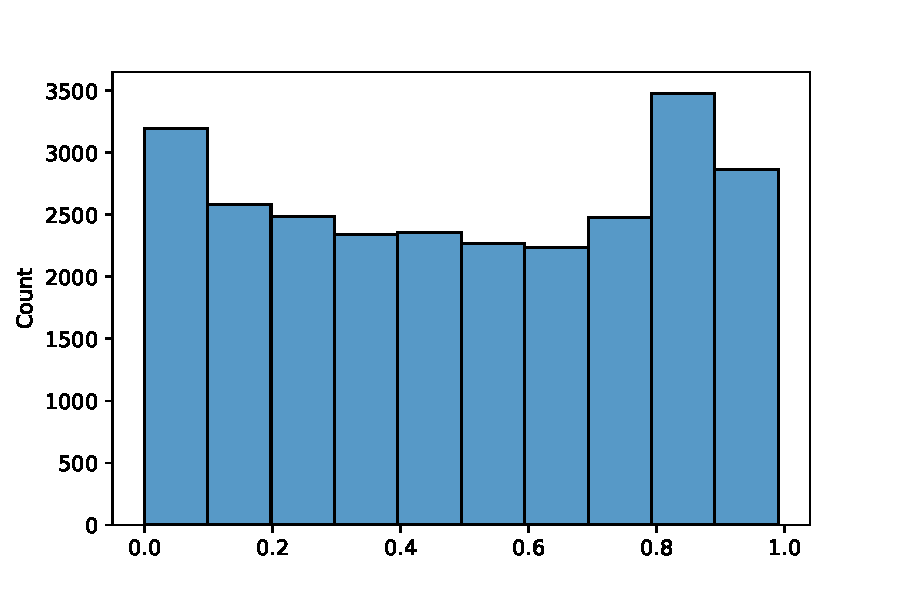
\includegraphics[width=0.45\textwidth]{plots/pit/pit_qrf.pdf} \label{fig:pit-qrf} }}
    \subfloat[\centering Nearest Neighbor Quantile Filters]{{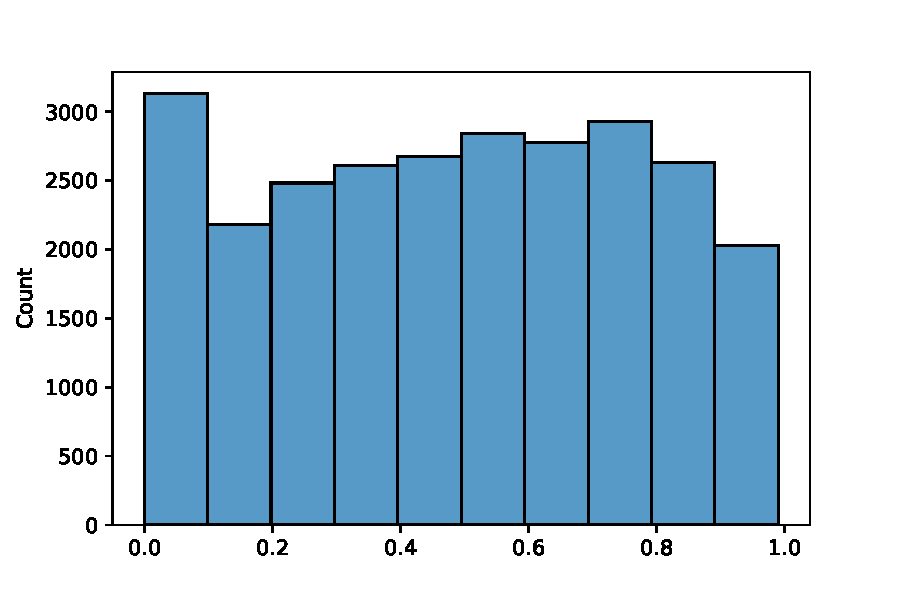
\includegraphics[width=0.45\textwidth]{plots/pit/pit_nnqf.pdf} \label{fig:pit-nnqf} }} \\
    \subfloat[\centering DeepAR]{{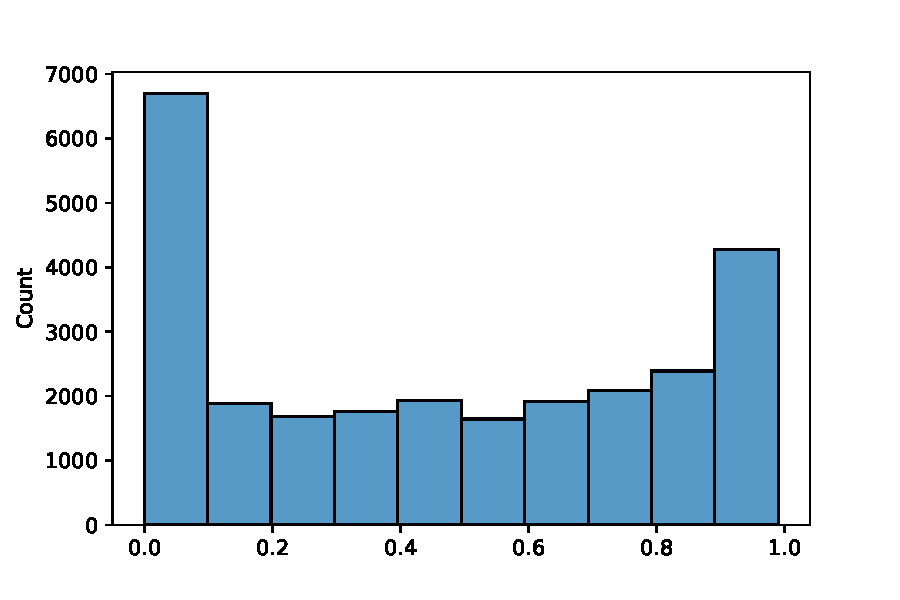
\includegraphics[width=0.45\textwidth]{plots/pit/pit_deepar.pdf} \label{fig:pit-deepar} }}
    \subfloat[\centering Spline Quantile Functions RNN]{{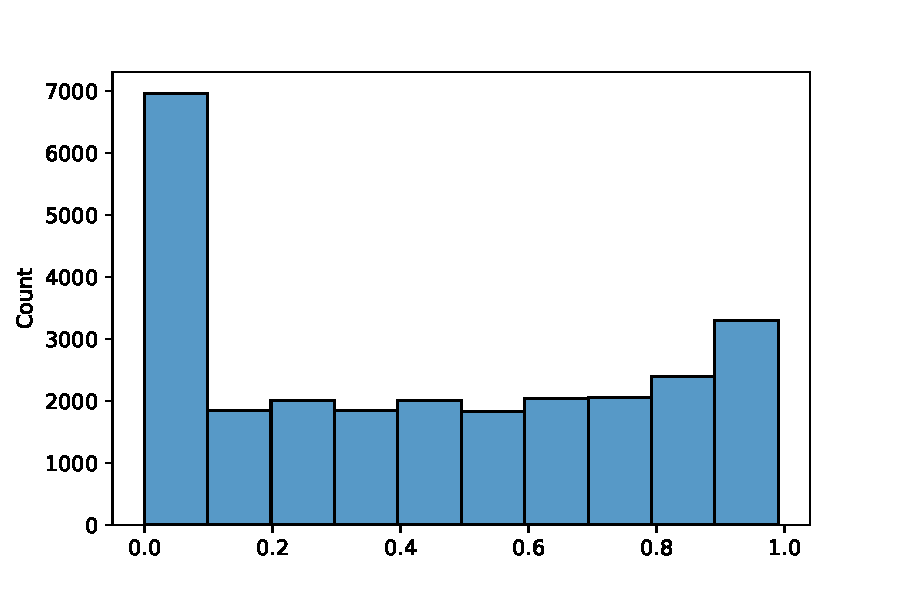
\includegraphics[width=0.45\textwidth]{plots/pit/pit_sqf-rnn.pdf} \label{fig:pit-sqf-rnn} }}
    \caption[PIT histograms]{Probability integral transform of each model. 
    If the distribution of the PIT looks like \(U(0,1)\), it's probabilistically calibrated.}%
    \label{fig:pit}%
\end{figure}

The PIT histograms broken down into each hour are shown in Figure \ref{fig:pit-qrf-by-hour}, Figure \ref{fig:pit-nnqf-by-hour}, 
Figure \ref{fig:pit-deepar-by-hour} and Figure \ref{fig:pit-sqf-rnn-by-hour}. 
The PIT histograms averaged over each hour are shown in Figure \ref{fig:pit}. 

One can observe that the PIT histogram of QRF (\ref{fig:pit-qrf}) and NNQF (\ref{fig:pit-nnqf}) are approximately 
\(U(0,1)\)-distributed but the forecasts during the night are overdispersed in the QRF case and 
skewed in the NNQF model.

The DeepAR and SQF-RNN model perform similarly: they are both skewed with a high density at \(0\). 
This means that the actual output lies often in the lower quantiles of the prediction. 